\documentclass[a4paper, 12pt]{article}
\usepackage{geometry}
\usepackage{graphicx}
\usepackage{mathtools}
\usepackage{listings}
\usepackage{float}
\usepackage[utf8]{inputenc}
\geometry{margin=1in}

\usepackage{color} %red, green, blue, yellow, cyan, magenta, black, white
\definecolor{mygreen}{RGB}{28,172,0} % color values Red, Green, Blue
\definecolor{mylilas}{RGB}{170,55,241}

\begin{document}

\section{Vergelijkende analyse van discreet equivalent}

\lstset{language=Matlab,%
    %basicstyle=\color{red},
    breaklines=true,%
    morekeywords={matlab2tikz},
    keywordstyle=\color{blue},%
    morekeywords=[2]{1}, keywordstyle=[2]{\color{black}},
    identifierstyle=\color{black},%
    stringstyle=\color{mylilas},
    commentstyle=\color{mygreen},%
    showstringspaces=false,%without this there will be a symbol in the places where there is a space
    numbers=left,%
    numberstyle={\tiny \color{black}},% size of the numbers
    numbersep=9pt, % this defines how far the numbers are from the text
    emph=[1]{for,end,break},emphstyle=[1]\color{red}, %some words to emphasise
    %emph=[2]{word1,word2}, emphstyle=[2]{style},    
}
\begin{lstlisting}
ts = 0.1;
c1 = tf([1], [1 1])
d1 = tf([ts], [1 -1+ts], ts)
d2 = tf([ts/(ts+1) 0], [1 -1/(ts+1)], ts)
d3 = tf([ts ts], [ts+2 -2+ts], ts)
d4 = tf([1-exp(-ts) +1-exp(-ts)], [2 -2*exp(-ts)], ts)
d5 = tf([1-exp(-ts)], [1 -exp(-ts)], ts)

step(c1, d1, d2, d3, d4, d5)
legend('c1', 'd1', 'd2', 'd3', 'd4', 'd5')
\end{lstlisting}

Dit is de broncode van het matlab script dat de stapresponsies geeft voor verschillende discrete equivalenten.\\
Deze code geeft volgend resultaat.

\begin{figure}[!h]
	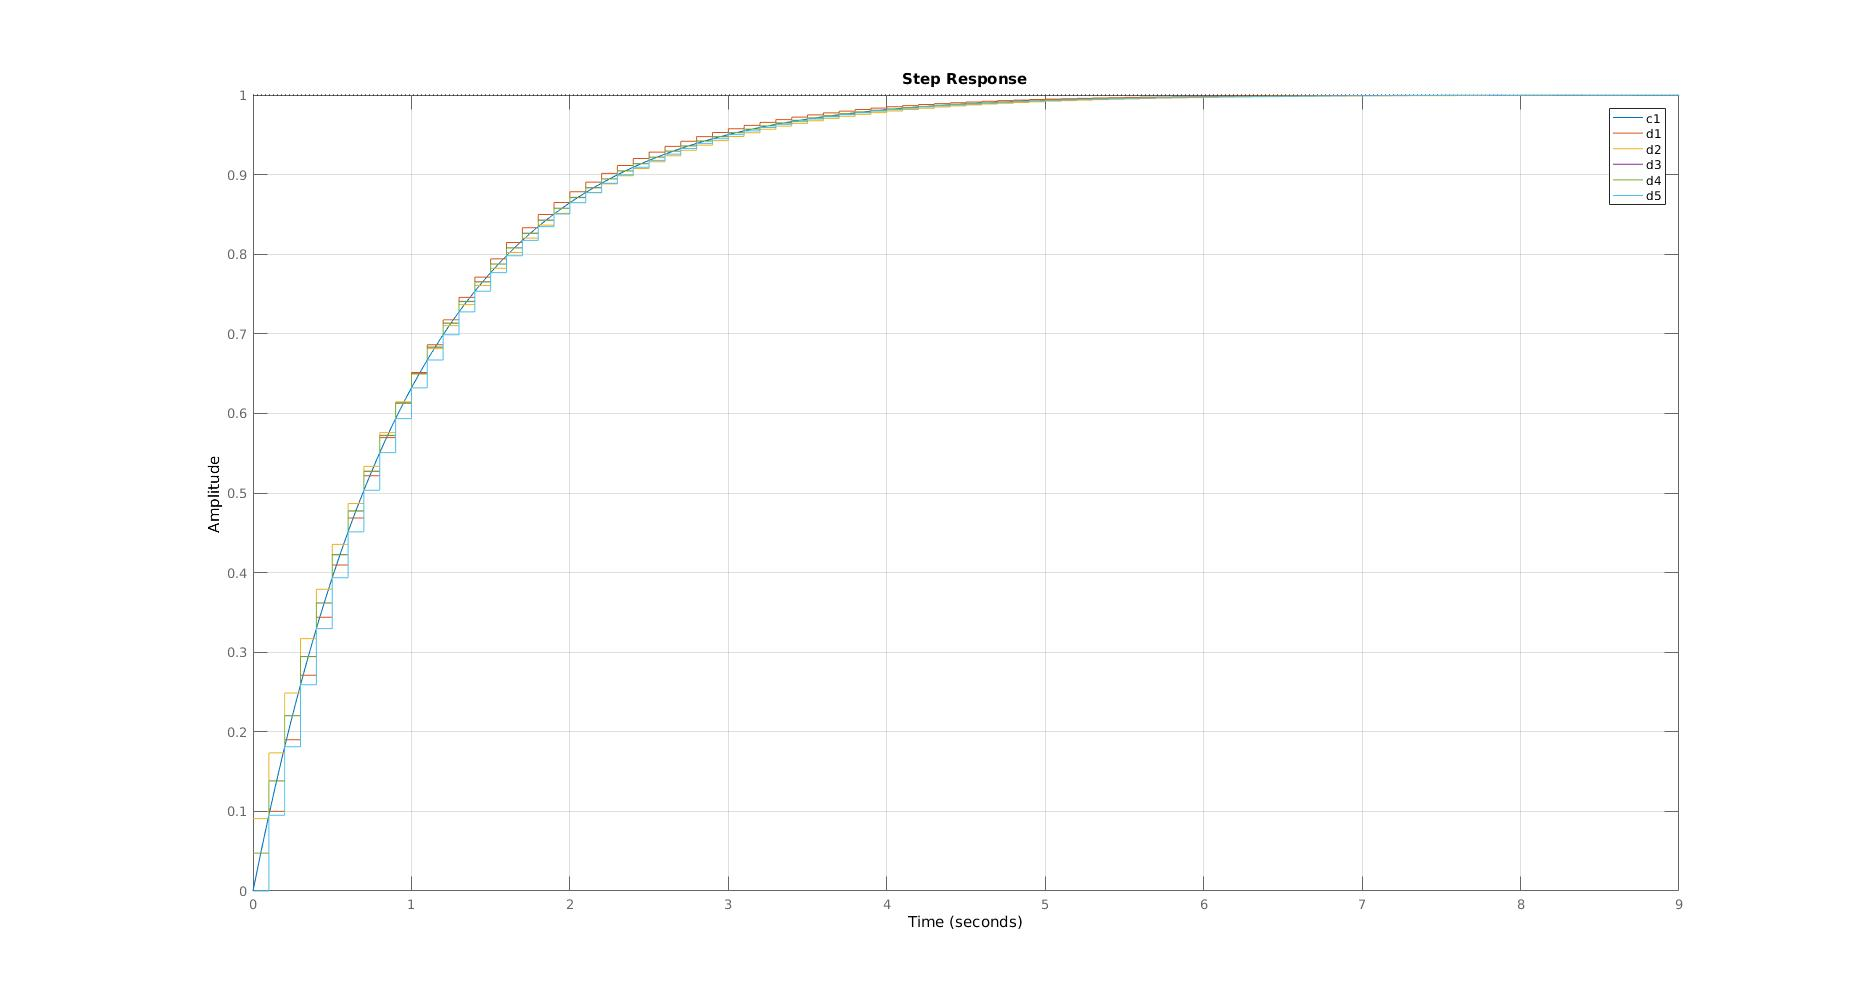
\includegraphics[width=1\linewidth]{Labo3_step_response.jpg}
	\caption{Stepresponse van het analoog en de 5 discrete systemen}
	\label{fig:Labo3_step_response}
\end{figure}

Op deze figuur zien we niet veel. Wat wel wel zien is dat ruw gezien alle discrete equivalenten het analoog systeem lijken te volgen.\\
Maar we gaan deze figuur toch in wat meer detail bekijken.

\begin{figure}[H]
	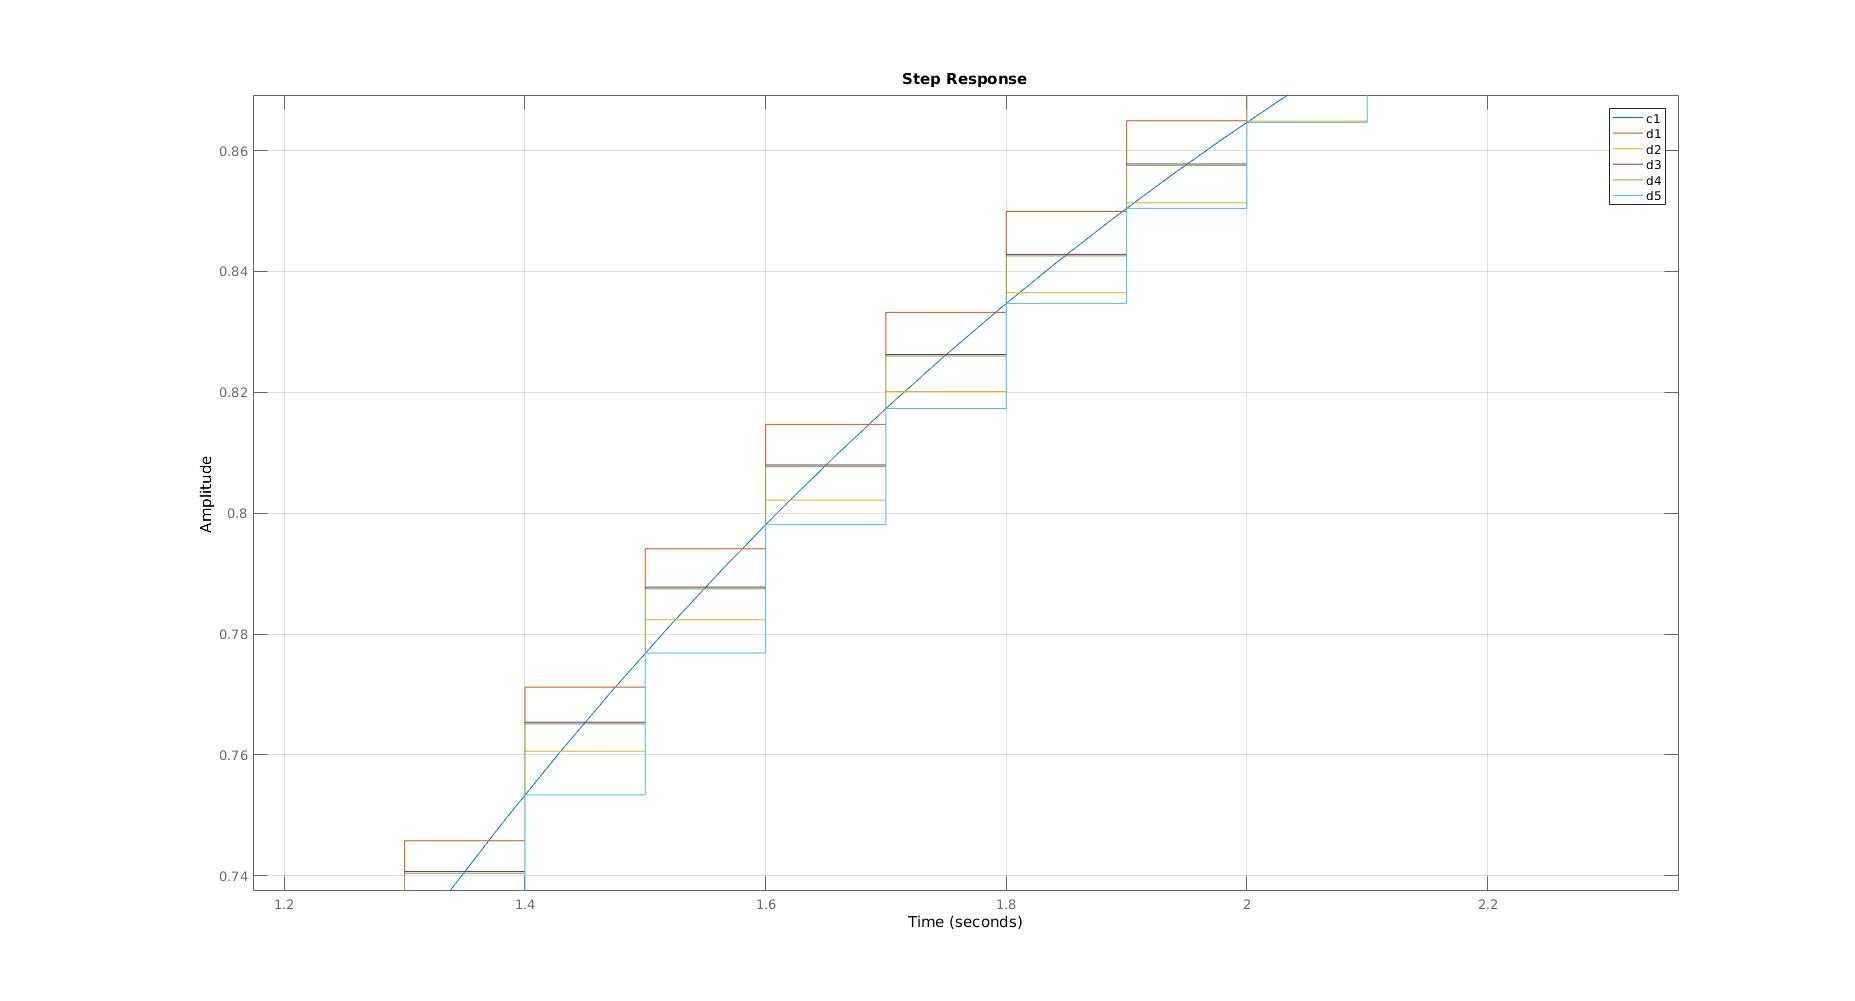
\includegraphics[width=1\linewidth]{Labo3_step_response2.jpg}
	\caption{ingezoomde stepresponse}
	\label{fig:Labo3_step_response_zoom}
\end{figure}

Figuur \ref{fig:Labo3_step_response_zoom} geeft een beter beeld op figuur \ref{fig:Labo3_step_response}. Met deze figuur zullen we dan ook een paar vaststellingen kunnen doen. \\

\underline{Welke 2 discrete equivalenten zijn bijna identiek?}\\
Als we goed naar de figuur kijken kunnen we zien dat systeem d3 en d4 bijna op elkaar vallen, en dus ook bij identiek zijn. Dit zijn respectievelijk het systeem met de Trapeziumregel en het systeem met de Nulpunten/polen-transformatie.\\

\underline{Welke discrete TF levert exacte digitale waarden op; dit is identiek aan de continue waarden?}\\

\underline{Welke twee discrete equivalenten geven een slechte benadering?}\\
De systemen die het meest aan de buitenkant liggen en dus de slechtste benadering geven zijn: d1 en d5. Deze systemen zijn respectievelijk het systeem met de voorwaartse integratieregel en het systeem met het Houdequivalent.

\end{document}